\documentclass[tikz]{standalone}
\usetikzlibrary{circuits.logic.US,calc}

\usepackage[caption=false]{subfig}
\usepackage{xcolor}
%\def\cellsize{0.425}

\colorlet{dot-color}{black!80}
\definecolor{clock1}{HTML}{86E291}
\definecolor{clock2}{HTML}{FFA5FA}
\definecolor{clock3}{HTML}{00C8BC}
\definecolor{clock4}{HTML}{F2F2F2}
\definecolor{fixed}{HTML}{000000}
\tikzset{cell size/.store in=\cellsize, cell size=0.45}
\tikzset{
  pics/gcell/.style = {
    code = {
      \coordinate (-center) at (0,0);
      
      \fill +(-\cellsize,-\cellsize) coordinate(-sw) 
      -- +(-\cellsize, \cellsize) coordinate(-nw)
      -- +( \cellsize, \cellsize) coordinate(-ne)
      -- +( \cellsize,-\cellsize) coordinate(-se)
      -- cycle;
      \coordinate (-swo) at ($ (-center)!0.5!(-sw) $);
      \coordinate (-nwo) at ($ (-center)!0.5!(-nw) $);
      \coordinate (-neo) at ($ (-center)!0.5!(-ne) $);
      \coordinate (-seo) at ($ (-center)!0.5!(-se) $);
      
      \coordinate (-south) at ($ (-sw)!.5!(-se) $);
      \coordinate (-north) at ($ (-nw)!.5!(-ne) $);
      \coordinate (-west)  at ($ (-sw)!.5!(-nw) $);
      \coordinate (-east)  at ($ (-se)!.5!(-ne) $);
      
      \fill[white] (-swo) let \p1=($ (-center)!.5!(-swo) $) in circle ({veclen(\x1,\y1)});
      \fill[white] (-nwo) let \p1=($ (-center)!.5!(-nwo) $) in circle ({veclen(\x1,\y1)});
      \fill[white] (-neo) let \p1=($ (-center)!.5!(-neo) $) in circle ({veclen(\x1,\y1)});
      \fill[white] (-seo) let \p1=($ (-center)!.5!(-seo) $) in circle ({veclen(\x1,\y1)});
      
      \ifnum#1=1\relax
      \fill[dot-color] (-swo) let \p1=($ (-center)!.32!(-swo) $) in circle ({veclen(\x1,\y1)});
      \fill[dot-color] (-neo) let \p1=($ (-center)!.32!(-neo) $) in circle ({veclen(\x1,\y1)});
      \else
      \ifnum#1=-1\relax
      \fill[dot-color] (-nwo) let \p1=($ (-center)!.32!(-nwo) $) in circle ({veclen(\x1,\y1)});
      \fill[dot-color] (-seo) let \p1=($ (-center)!.32!(-seo) $) in circle ({veclen(\x1,\y1)});
      \else
      \fill[dot-color] (-swo) let \p1=($ (-center)!.22!(-swo) $) in circle ({veclen(\x1,\y1)});
      \fill[dot-color] (-nwo) let \p1=($ (-center)!.22!(-nwo) $) in circle ({veclen(\x1,\y1)});
      \fill[dot-color] (-neo) let \p1=($ (-center)!.22!(-neo) $) in circle ({veclen(\x1,\y1)});
      \fill[dot-color] (-seo) let \p1=($ (-center)!.22!(-seo) $) in circle ({veclen(\x1,\y1)});
      \fi
      \fi
    }
  },
  pics/gcell/.default={0},,
}

\begin{document}
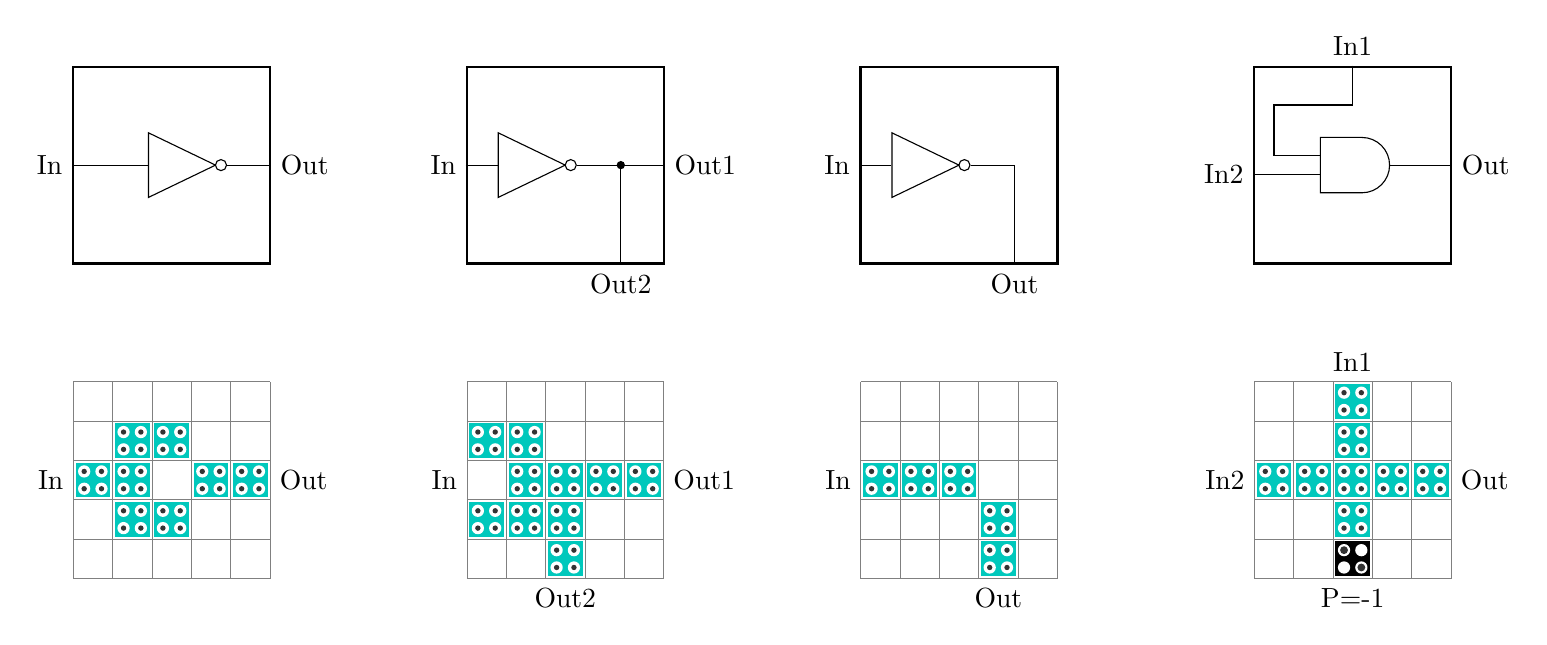
\begin{tikzpicture}

\begin{scope}[
circuit logic US,
large circuit symbols,
border/.style={minimum size=2.5cm, rectangle, draw, thick}
]

\begin{scope}
\node(b)[border] {};
\node(n) [not gate]  {};
\draw (b.west) node[left]{In} -- (n.input)
      (n.output) -- (b.east) node[right]{Out};
\end{scope}

\begin{scope}[xshift=5cm]
\node(b)[border] {};
\node(n)[not gate, anchor=east] {};
\draw (b.west) node[left]{In} -- (n.input);
\coordinate (fanpoint) at ($(n.output)!.5!(b.east)$);
\draw (n.output) -- (b.east) node[right]{Out1}
      (n.output) -| ($(b.south west)!(fanpoint)!(b.south east)$) node[below]{Out2}
;
\fill (fanpoint) circle[radius=1.5pt];
\end{scope}

\begin{scope}[xshift=10cm]
\node(b)[border]{};
\node(n)[not gate, anchor=east]{};
\draw (b.west) node[left]{In} -- (n.input);
\draw (n.output) -| ($(b.south west)!($(n.output)!.5!(b.east)$)!(b.south east)$) node[below]{Out};
\end{scope}

\begin{scope}[xshift=15cm]
\node(b)[border]{};
\node(a)[and gate ]{};
\draw(a.output)--(b.east)node[right]{Out};
\draw (b.north) node[above]{In1} -- ++(0,-0.5cm) -- ++(-1cm,0) |- (a.input 1)
      (a.input 2) -- ($(b.north west)!(a.input 2)!(b.south west)$) node[left]{In2}
;
\end{scope}

\end{scope}%circuit scope

\begin{scope}[cell size=0.22cm, x=0.5cm, y=0.5cm, yshift=-5cm]

\begin{scope}[xshift=-1cm]
\draw[help lines, step=0.5cm, xshift=-0.25cm, yshift=-0.25cm] (0,0) grid (5,5);
\foreach \coord in {{0,2},{1,1},{1,2},{1,3},{2,1},{2,3},{3,2},{4,2}} \path (\coord)pic[clock3]{gcell};

\path (0,2)node[left=0.25cm]{In}
      (4,2)node[right=0.25cm]{Out}
;
\end{scope}

\begin{scope}[xshift=4cm]
\draw[help lines, step=0.5cm, xshift=-0.25cm, yshift=-0.25cm] (0,0) grid (5,5);
\foreach \coord in {{0,1},{0,3},{1,1},{1,2},{1,3},{2,0},{2,1},{2,2},{3,2},{4,2}} \path (\coord) pic[clock3]{gcell};

\path (0,2)node[left=0.25cm]{In}
      (4,2)node[right=0.25cm]{Out1}
      (2,0)node[below=0.25cm]{Out2}
;
\end{scope}
 
\begin{scope}[xshift=9cm]
\draw[help lines, step=0.5cm, xshift=-0.25cm, yshift=-0.25cm] (0,0) grid (5,5);
\foreach \coord in {{0,2},{1,2},{2,2},{3,0},{3,1}} \path (\coord) pic[clock3]{gcell};

\path (0,2)node[left=0.25cm]{In}
      (3,0)node[below=0.25cm]{Out}
;
\end{scope}

\begin{scope}[xshift=14cm]
\draw[help lines, step=0.5cm, xshift=-0.25cm, yshift=-0.25cm] (0,0) grid (5,5);
\foreach \coord in {{0,2},{1,2},{2,1},{2,2},{2,3},{2,4},{3,2},{4,2}} \path (\coord) pic[clock3]{gcell};
\path (2,0)node[below=0.25cm]{P=-1} pic[fixed]{gcell=-1};

\path (2,4) node[above=0.25cm]{In1}
      (0,2) node[left=0.25cm]{In2}
      (4,2) node[right=0.25cm]{Out}
;
\end{scope}

\end{scope}%cell scope


\end{tikzpicture}
\end{document}
